\section{Activity Diagram}

Activity diagrams provide a visual representation of the workflow and business processes within a system. For Jadwal, the activity diagram maps out the user's journey through the application, from authentication to daily interactions, illustrating the various paths and decision points users encounter. This diagram is particularly important as it demonstrates how different features of Jadwal—such as calendar management, WhatsApp integration, and conflict resolution—interconnect in actual usage.

An activity diagram is shown in Figure~\ref{fig:activity-diagram} above, and it illustrates the flows the user of the app can take. It starts with the authentication which supports both Google and Email. We call it authentication because we don't let the user think whether he has an account or not, we just ask them for the email, or Google account, and the rest is handled by the system. This makes the experience easy for the user, and especially with the user of Magic Links and OAuth, users don't need to memorize passwords to access Jadwal. Even though this method is easier for the user than other methods, it doesn't offer lower security. In fact, it is even more secure than other methods since the challenge allows the user to prove they own an account without needing to provide a password they make.

Then after the token is verified, a check is done to see if the user has a calendar or not. If the user has a calendar, we just move on, but if they don't have one, we create one and then move on. Here the user is inside the app and has two options, he can either view the calendar or open the settings page. When he views the calendar, he can view an event, or add one.

After any of the previous two steps, the user can go back to view calendar or open settings page. If the choose to open settings page, they have three actions available. They can add their Jadwal calendar account to iOS calendar accounts on their device, connect WhatsApp, schedule prayer times, or logout. 

Starting with adding adding the Jadwal calendar account, the user can initiate the process by clicking on a button. Then the device installs a `.mobileconfig' file that sets the credentials on the user's device with their permission. This `.mobileconfig' is what we call a provisining profile, and it allows you to change phone settings with good user experience, since asking users to enter three pieces of information and navigating alot of pages just to add a calendar account will result in them hating the app.

Then with the connecting a WhatsApp account feature. After a successful connection of the user's WhatsApp account, the system will start to extract events from the user's WhatsApp account automatically. If any conflicts arise after adding an event to the calendar, the system suggests a conflict resolution, and the user can take action by managing the scheduling conflict. But if no conflicts arise, the system just continues normally.

The flows above allows the user to continue using the app and doing other things with their account but the last action will block you from doing this. The logout action  terminates the session and the user is logged out of the app. This is an end state, and you need to start again from the start to be able to use the app again.

\begin{figure}[!h]
    \centering
    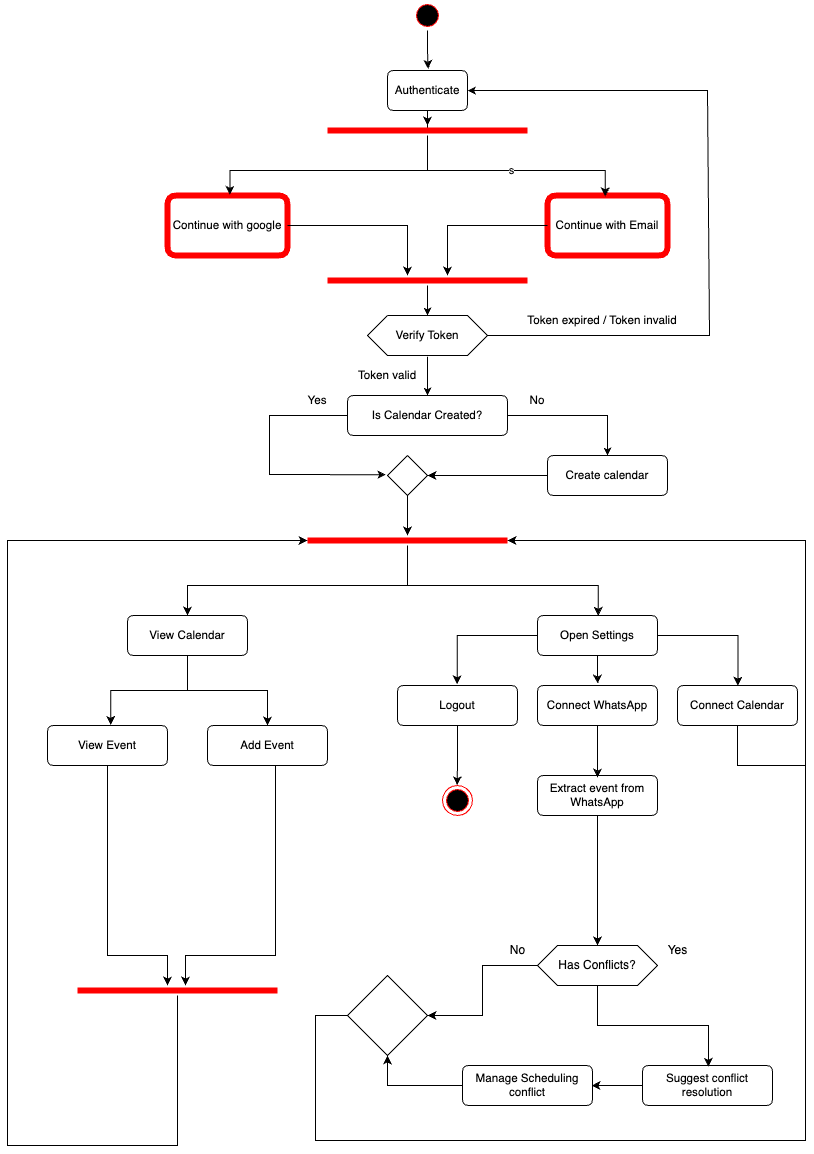
\includegraphics[width=0.9\textwidth]{images/activity-diagram.png}
    \caption{Activity Diagram of Jadwal}
    \label{fig:activity-diagram}
\end{figure}